\ifdefined\activerhandout 
\documentclass[12pt,aspectratio=1610,handout]{beamer}
\else
\documentclass[12pt,aspectratio=1610]{beamer}
\fi

%\usepackage[french]{babel} %=> erreur avec les tikz du moteur
\usepackage[T1]{fontenc}
\usepackage[utf8]{inputenc}
\usepackage{lmodern}
\usepackage{hyperref}
\usepackage{smartdiagram}
\usepackage{tikz}
\usepackage{animate}
\usepackage{tikzpeople}
\usepackage{appendixnumberbeamer}
\usepackage[labelformat=empty]{caption}
%\usepackage{pictochrono}
\usepackage{fontawesome5}
\usepackage{awesomebox}

\usetheme{Warsaw}
\setbeamertemplate{page number in head/foot}[totalframenumber]

\newcommand{\anglais}[1]{(\textit{\color{blue}#1})}
\newcommand{\legende}[2]{\caption[#1 (Source : \cite{#2})]{#1}}
\newcommand{\histoire}[1]{\begin{awesomeblock}{2pt}{\faBook}{black!75}#1\end{awesomeblock}}
\newcommand{\info}[1]{\begin{awesomeblock}{2pt}{\faInfoCircle}{black!75}#1\end{awesomeblock}}
\newcommand{\question}[1]{\begin{awesomeblock}{2pt}{\faQuestionCircle}{black!75}#1\end{awesomeblock}}
\newcommand{\alerte}[1]{\begin{awesomeblock}{2pt}{\faExclamationCircle}{black!75}#1\end{awesomeblock}}
\newcommand{\astuce}[1]{\begin{awesomeblock}{2pt}{\faLightbulb}{black!75}#1\end{awesomeblock}}
\newcommand{\exemple}[1]{\begin{awesomeblock}{2pt}{\faSearch}{black!75}#1\end{awesomeblock}}
\newcommand{\definitionAConnaitre}[1]{\begin{awesomeblock}{2pt}{\faCog}{black!75}#1\end{awesomeblock}}

\newcommand{\qmcBia}[7]{
%1 : titre slide
%2 : numéro de la bonne réponse
%3 : Inititulé de la question
%4, 5, 6, et 7 : propositions de réponse
\begin{frame}{#1}
\begin{awesomeblock}{2pt}{\faQuestion}{black!75}
#3
	\begin{enumerate}
	\ifnum#2=1
		\only<1>{\item #4}
		\only<2>{\item \textbf{#4}}
	\else
		\item #4
	\fi
	\ifnum#2=2
		\only<1>{\item #5}
		\only<2>{\item \textbf{#5}}
	\else
		\item #5
	\fi
	\ifnum#2=3
		\only<1>{\item #6}
		\only<2>{\item \textbf{#6}}
	\else
		\item #6
	\fi
	\ifnum#2=4
		\only<1>{\item #7}
		\only<2>{\item \textbf{#7}}
	\else
		\item #7
	\fi
	\end{enumerate}
	\pause
\end{awesomeblock}
\end{frame}
}

\subtitle{BIA - Brevet d'Initiation Aéronautique}
\author{Clément \textsc{Vermot-Desroches}}
\institute{Collège Aliénor d'Aquitaine\\Martignas-sur-Jalle}
\date{\today}

%\AtBeginSection[]
%{
%    \begin{frame}
%        %\frametitle{Table of Contents}
%        \tableofcontents[currentsection]
%    \end{frame}
%}

\AtBeginSubsection[]
{
    \begin{frame}
        %\frametitle{Table of Contents}
        \tableofcontents[currentsection,currentsubsection]
    \end{frame}
}
\input{commun/video.tex}

\title[Séance 3 - Aérodynamique]{Séance 3 \\ Aérodynamique}

\begin{document}
 \begin{frame}
 \titlepage
 \end{frame}
 
 \begin{frame}
 \tableofcontents
 \end{frame}
 
 \section{Portance et trainée}
 \subsection{La portance}
	\begin{frame}{Portance - Question}
	
	\question{On passe la main par la fenêtre d'une voiture en mouvement. Quels effets peut-on ressentir ?}
	\pause
	\question{Si on modifie l'inclinaison de la main, que se passe t'il ?}
	\end{frame}	 
	
	\begin{frame}{Les forces sur un aéronef}
		\begin{figure}[H]
			\only<1>{\includegraphics[scale=1.2]{imgPresentations/forces.pdf}}
  			\only<2>{\includegraphics[scale=1.2]{04-Aerodynamique/img/forces.pdf}}	
  			\legende{Les 4 forces}{img:forces}	
  			\pause
		\end{figure}
	\end{frame}
	
	\begin{frame}{Définitions autour de l'aile}
		\begin{figure}[H]
  			\includegraphics[scale=0.5]{04-Aerodynamique/img/profilAile.pdf}
  			\legende{Le profil d'une aile}{img:profilAile}	
		\end{figure}
	\end{frame}	
	
	\begin{frame}{Pression autour d'un profil d'aile}
		\begin{figure}[H]
  			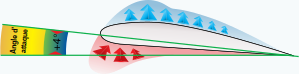
\includegraphics[scale=1.7]{04-Aerodynamique/img/pressionProfilSelonAngleAttaque4deg.pdf}
  			\legende{Pression autour d'un profil d'aile}{img:pressionProfilSelonAngleAttaque4deg}	
		\end{figure}
		\pause
		\begin{itemize}
			\item sur l'extrados, l'air est accéléré : la pression baisse
			\item sur l'intrados, l'air rencontre un obstacle : il est ralenti : la pression augmente
			\item 70~\% de la portance est due à l'aspiration sur l'extrados
		\end{itemize}
	\end{frame}
	
	\begin{frame}{Relation incidence/portance}
		\begin{figure}[H]
  			\includegraphics[scale=0.80]{04-Aerodynamique/img/portanceTraineeFinesse_portance.pdf}
  			\legende{Courbe de la portance en fonction de l'incidence}{img:portanceTraineeFinesse}	
		\end{figure}
	\end{frame}
	
	\subsection{La trainée}
	\begin{frame}{Trainée}
	En physique, un phénomène souhaité est souvent accompagné d'un ou plusieurs phénomènes parasites, indésirable.
	
	\pause
	
	En aérodynamique, la portance s'accompagne d'une force qui va résister à l'avancement de l'aéronef : la trainé.
	
	\end{frame}
	
	\begin{frame}{Relation incidence/trainée}
		\begin{figure}[H]
  			\includegraphics[scale=0.80]{04-Aerodynamique/img/portanceTraineeFinesse_trainee.pdf}
  			\legende{Courbe de la trainée en fonction de l'incidence}{img:portanceTraineeFinesse}	
		\end{figure}
	\end{frame}
	
	\begin{frame}{Décrochage}
		\begin{figure}[H]
  			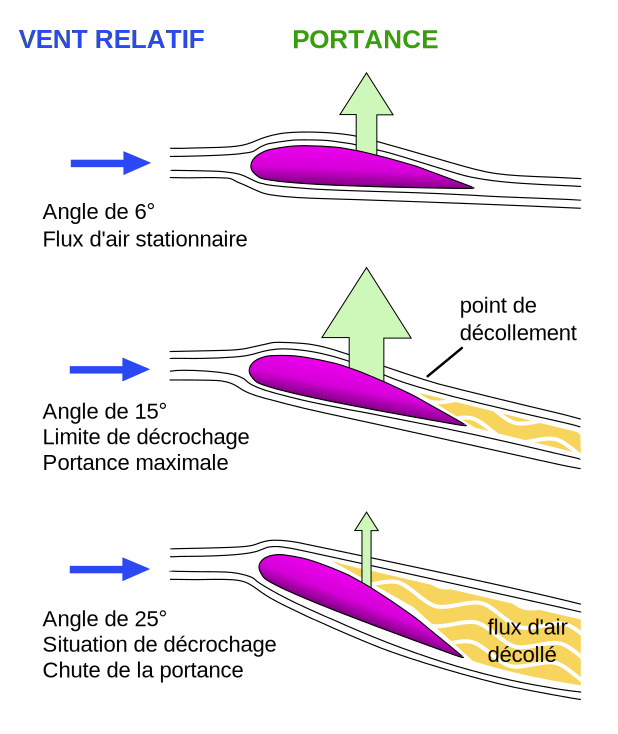
\includegraphics[scale=0.42]{04-Aerodynamique/img/portanceDecrochage.pdf}
  			\legende{}{img:portanceDecrochage}	
		\end{figure}
	\end{frame}
	
	\begin{frame}{Les équations}
	
	\begin{columns}
 		\begin{column}{0.5\textwidth}
 		\begin{center}
		La portance :
		
		~		
		
		\huge{$Z = \dfrac{1}{2}\rho S V^2 Cz$}
		\end{center}
		\end{column}
		\begin{column}{0.5\textwidth}
		\begin{center}
		La trainée :
		
		~		
		
		\huge{$X = \dfrac{1}{2}\rho S V^2 Cx$}
		\end{center}
		\end{column}
	\end{columns}
	
	~\newline
	avec \begin{itemize}
	\item $\rho$ : densité de l'air en $kg/m^3$ ($\sim 1,2~kg/m^3$)
	\item $S$ : surface de l'aile en $kg$
	\item $V$ : vitesse en $m/s$
	\item $Cz$ : coefficient de portance (sans unité)
	\item $Cx$ : coefficient de trainée (sans unité)
	\end{itemize}
	
	\end{frame}
	
	\begin{frame}{Comment expliquer ces tourbillons ?}
	\begin{figure}[H]
	\only<1>{\scalebox{.35}{\includegraphics[page=1, scale=0.4]{04-Aerodynamique/img/vortex}}
	\legende{Vortex}{img:vortex}}
  	\only<2>{\scalebox{.35}{\embedvideo*{\includegraphics[page=1, scale=0.4]{04-Aerodynamique/img/vortex}}{04-Aerodynamique/img/vortex.ogv}}
  	\legende{Vortex}{video:vortex}}
	\end{figure}

	\pause
	\end{frame}
	
	\begin{frame}{Tourbillons marginaux}
	\begin{columns}
 	\begin{column}{0.4\textwidth}
		\begin{figure}[H]
  			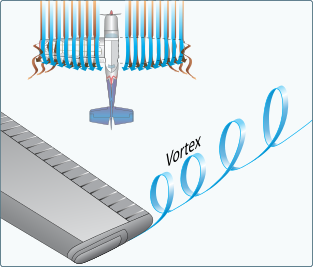
\includegraphics[width=1.0\textwidth]{04-Aerodynamique/img/vortexSchema.pdf}
  			\legende{Création de vortex}{img:vortexSchema}	
		\end{figure}
	\end{column}	
 	\begin{column}{0.6\textwidth}
	Les tourbillons marginaux sont crées par "l'aspiration" de l'air en surpression de l'intrados vers l'air en dépression sur l'extrados
	\pause
 	Pour les réduire, on peut :
 		\begin{itemize}
 			\item augmenter l'allongement de l'aile (planeur, avions de ligne)
 			\pause
 			\item ajouter des winglets en bout d'aile
 		\end{itemize}
 	\end{column}
 	\end{columns}
	\end{frame}
	
	\begin{frame}{Tourbillons marginaux}
		\begin{figure}[H]
  			\includegraphics[width=0.75\textwidth]{04-Aerodynamique/img/Falcon7XWinglet.jpg}
  			\legende{Falcon 7X avec winglets}{img:Falcon7XWinglet}	
		\end{figure}
	\end{frame}
	
	\begin{frame}{Finesse}
		\begin{figure}[H]
  			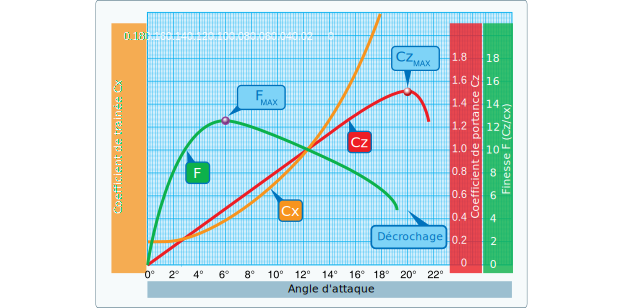
\includegraphics[scale=0.80]{04-Aerodynamique/img/portanceTraineeFinesse.pdf}
  			\legende{Courbes de la finesse en fonction de l'incidence}{img:portanceTraineeFinesse}	
		\end{figure}
	\end{frame}
	
	\begin{frame}{Polaire d'une aile}
	\begin{columns}
 	\begin{column}{0.4\textwidth}
		\begin{figure}[H]
  			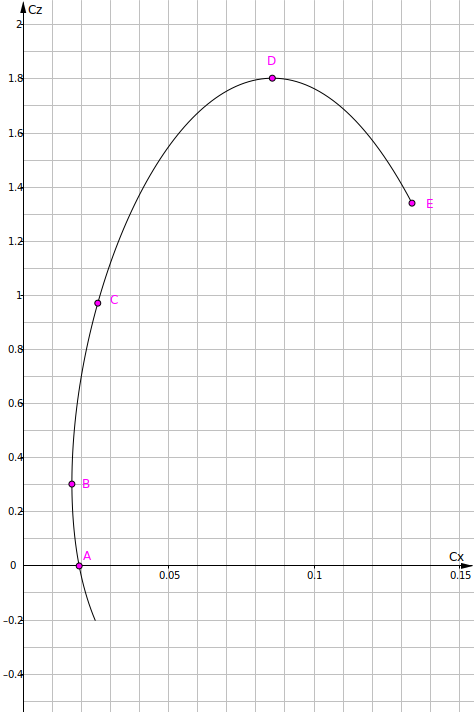
\includegraphics[scale=0.35]{04-Aerodynamique/img/polaireAile.pdf}
  			\legende{Polaire d'une aile}{img:polaireAile}	
		\end{figure}
	\end{column}	
 	\begin{column}{0.6\textwidth}
	Obtenue en traçant la portance $C_z$ en fonction de la trainée $C_x$. 
	\pause
 	
 		\begin{itemize}
 			\item $A$ : $Cz = 0 \Rightarrow$ portance nulle
 			\item $B$ : trainée $C_x$ minimale
 			\item $C$ : $\dfrac{C_z}{C_x}$ minimum $\Rightarrow$ finesse maximale
 			\item $D$ : portance $C_z$ maximale
 			\item $E$ : décrochage
 		\end{itemize}
 	\pause
 	\alerte{Le décrochage se fait toujours à la même incidence}
 	\end{column}
 	\end{columns}
	\end{frame}
	
	\section{Les dispositifs hypersustentateurs}
	\begin{frame}{Les dispositifs hypersustentateurs}
	On a vu que pour augmenter la portance, un pilote pourrait agir :
	\begin{itemize}
		\item sur la vitesse
		\item sur l'incidence
	\end{itemize}
	
	\question{Ne pourrait-on pas agir sur la forme ou la surface de l'aile ?}
	\pause
	\question{Pourquoi chercher à modifier ces 2 paramètres ?}
	
	\end{frame}
	
	\begin{frame}{Becs et volets}
	\begin{figure}[H]
  			\includegraphics[width=0.75\textwidth]{04-Aerodynamique/img/voletsBecs.jpg}
  			\legende{Volets et becs sur un A318}{img:voletsBecs}	
		\end{figure}
	\end{frame}
	
	\begin{frame}{Différents types dispositifs hypersustentateurs}
	\begin{columns}
 	\begin{column}{0.5\textwidth}
		\begin{figure}[H]
  			\includegraphics[width=1.0\textwidth]{04-Aerodynamique/img/hypersustentateurs/voletsDeCourbure.pdf}
  			\legende{Volets de courbure}{img:voletsDeCourbure}	
		\end{figure}
	\end{column}	
 	\begin{column}{0.5\textwidth}
		Augmente la courbure, donc le Cz
 	\end{column}
 	\end{columns}
 	\pause
 	\begin{columns}
 	\begin{column}{0.5\textwidth}
		\begin{figure}[H]
  			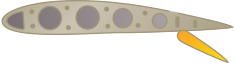
\includegraphics[width=1.0\textwidth]{04-Aerodynamique/img/hypersustentateurs/voletDIntrados.pdf}
  			\legende{Volets d'intrados}{img:voletDIntrados}	
		\end{figure}
	\end{column}	
 	\begin{column}{0.5\textwidth}
		Augmente la courbure, donc le Cz. Augmente énormément la trainée
 	\end{column}
 	\end{columns}
	\end{frame}
	
	\begin{frame}{Différents types dispositifs hypersustentateurs}
	\begin{columns}
 	\begin{column}{0.5\textwidth}
		\begin{figure}[H]
  			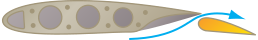
\includegraphics[width=1.0\textwidth]{04-Aerodynamique/img/hypersustentateurs/voletFowler.pdf}
  			\legende{Volets Fowler}{img:voletFowler}	
		\end{figure}
	\end{column}	
 	\begin{column}{0.5\textwidth}
		Augmente la surface de l'aile
 	\end{column}
 	\end{columns}
 	\pause
 	\begin{columns}
 	\begin{column}{0.5\textwidth}
		\begin{figure}[H]
  			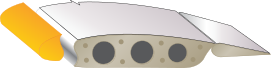
\includegraphics[width=1.0\textwidth]{04-Aerodynamique/img/hypersustentateurs/becs.pdf}
  			\legende{Becs de bord d'attaque}{img:becs}	
		\end{figure}
	\end{column}	
 	\begin{column}{0.5\textwidth}
		Augmente la surface de l'aile
 	\end{column}
 	\end{columns}
 	
 	\info{Quand les volets et les becs sont rentrés, on dit que l'aile est en configuration \textbf{lisse}}
	\end{frame}
	
	\begin{frame}{Les dispositifs hypersustentateurs}
	
	\question{Pourquoi a t'on rendu ces dispositifs mobiles ?}
	\pause
	
	\begin{itemize}
		\item Toute augmentation de la portance d'une aile se fait au prix de l'augmentation de la trainée
		\pause
		\item On veut pouvoir voler lentement à certaines phases du vol
		\pause
		\item Mais rapidement en croisière, en limitant la consommation de carburant
	\end{itemize}
	\pause
	$\Rightarrow$ les dispositifs hypersustentateurs sont utilisés uniquement quand on veut voler plus lentement
	
	\end{frame}
 
 
\appendix 
\section{QCM}
\qmcBia{Aérodynamique, aérostatique et principes du vol}
{2}{En soufflerie, si on multiplie par 3 la vitesse du vent relatif, la valeur de la portance est :}
{multipliée par 3}
{multipliée par 9}
{multipliée par 6}
{multipliée par 12} 
{Expression de la portance : $Z = \dfrac{1}{2}\rho S V^2 Cz$. Le facture vitesse est au carré, donc si on multiplie V par 3, la portance est multipliée par $3^2 = 9$.}

\qmcBia{Aérodynamique, aérostatique et principes du vol}
{3}{L'origine de la sustentation de l'aile résulte de l'apparition :}
{d'une dépression à l'extrados et à l'intrados}
{d'une surpression à l'intrados et à l'extrados}
{d'une dépression à l'extrados et d'une surpression à l'intrados}
{d'une surpression à l'extrados et d'une dépression à l'intrados} 
{}

\qmcBia{Aérodynamique, aérostatique et principes du vol}
{3}{L'incidence d'une aile est positive lorsque :}
{l'écoulement est parallèle à la corde du profil}
{l'écoulement attaque le profil du côté de l'extrados}
{l'écoulement attaque le profil du côté de l'intrados}
{l'aéronef est en vol dos stabilisé} 
{}

\qmcBia{Aérodynamique, aérostatique et principes du vol}
{1}{Le profil d'une aile est lisse lorsque :}
{les becs de bord d'attaque et les volets sont rentrés}
{les becs de bord d'attaque sont rentrés et les volets sont sortis}
{les becs de bord d'attaque sont sortis et les volets sont rentrés}
{les becs de bord d'attaque et les volets sont sortis} 
{}

\qmcBia{Aérodynamique, aérostatique et principes du vol}
{4}{Les dispositifs hypersustentateurs ont pour but :}
{de diminuer la portance à vitesse élevée (par exemple : pour une descente d'urgence)}
{d'augmenter la vitesse de décrochage pour certaines manœuvres}
{de diminuer la traînée pour certaines man\oe uvres}
{de diminuer la vitesse de décrochage dans certaines phases de vol (par exemple : au décollage et à l'atterrissage)} 
{}
 
\ifdefined\activerbibliobeamer
\begin{frame}[allowframebreaks]
\frametitle{Bibliographie}
\printbibliography
%\nocite{*}
\end{frame}
\fi 
 
\end{document}
